\section{Methoden}

\begin{frame}
	\frametitle{Methoden}
	
	\textbf{Kerndichteschätzung:}
	\begin{itemize}
		\item Annahme: Daten wurden von 'Modell' generiert
		\item Gegeben Trainingsdaten: wie wahrscheinlich ist ein Datenpunkt?
		\item $\hat{f}_h(x) = \frac{1}{nh}\sum_{i=1}^{n} K(\frac{x - x_i}{h})$
		\item $K$ ist die Kernelfunktion (f\"ur gew\"ohnlich Gauss)
		\item $h$ ist die \textit{Bandbreite}
	\end{itemize}
\end{frame}

\begin{frame}
	\frametitle{Methoden}
	
	\begin{itemize}
		\item Beeinflusst den Grad der Gl\"attung des Kernels
		\item Optimale Bandbreite nicht geschlossen berechenbar
	\end{itemize}
	
	\begin{figure}[p]
		\centering
		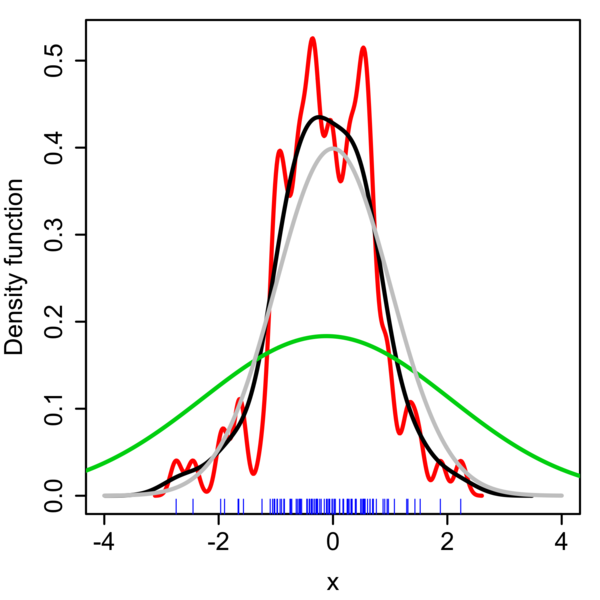
\includegraphics[width=0.4\textwidth]{figures/Bandwidth_comparison.png}
		\caption{Vergleich verschiedener Bandbreiten}
		\label{fig:bandwidth}
	\end{figure}
\end{frame}

\begin{frame}
	\frametitle{Methoden}
	
	\textbf{Parzen-Window-Klassifikator:}
	\begin{itemize}
		\item Nutze KDE zur Klassifikation
		\item F\"ur jede Klasse separate KDE
		\item $p(c | x) \propto \hat{f}_h^c(x) \cdot \theta_c$
	\end{itemize}
		
	\begin{figure}[p]
		\centering
		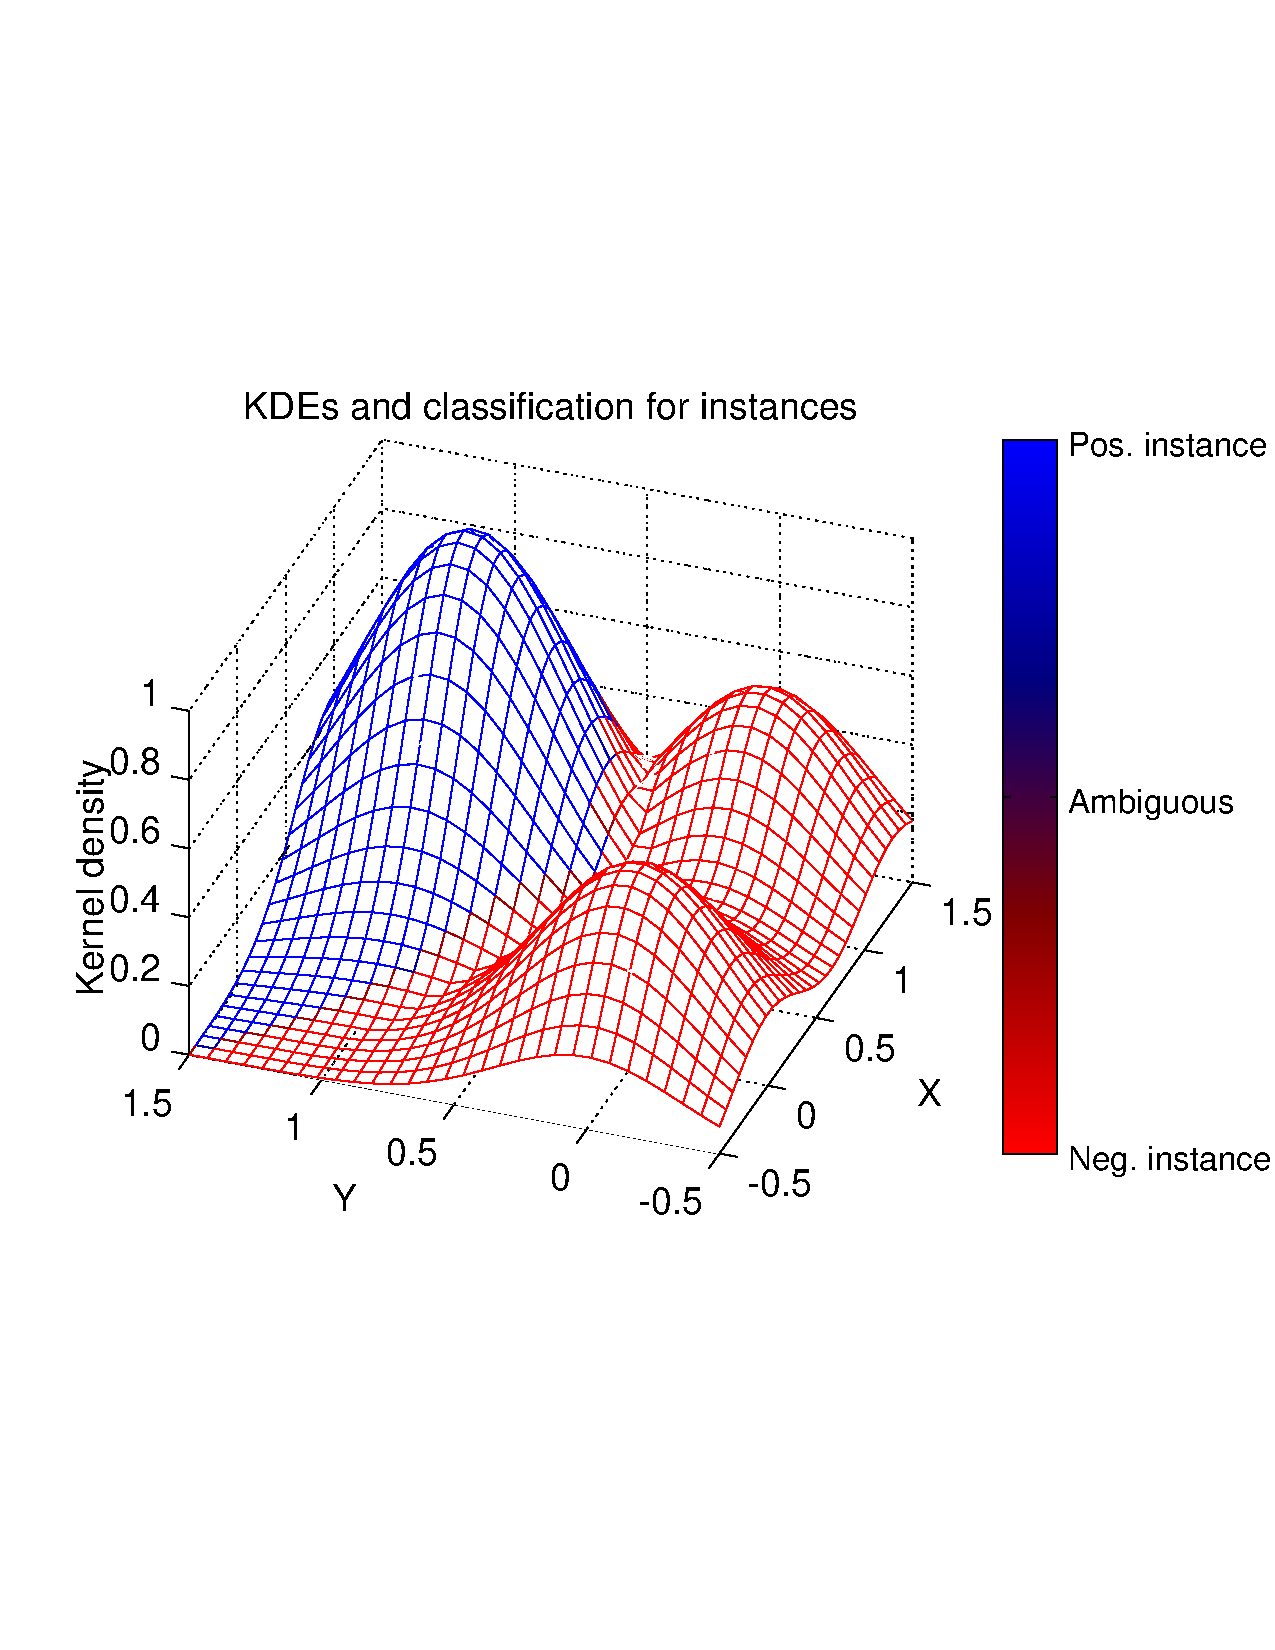
\includegraphics[trim = 0cm 6cm 0cm 5cm, clip = true, width = 0.6\textwidth]{figures/KDE3inst.pdf}
		\caption{}
		\label{fig:parzenwindow}
	\end{figure}
\end{frame}

\begin{frame}
	\frametitle{Methoden}
	
	\textbf{Silverman's Rule of Thumb:}
	\begin{itemize}
		\item Empirisch ermittelte Faustregel f\"ur Gausskernel
		\item Basiert auf geschätzter Varianz
		\item Nur Diagonalmatrix!
	\end{itemize}
	
\end{frame}

\begin{frame}
	\frametitle{Methoden}
		
	\textbf{Monte Carlo Markov Chain:}
	\begin{itemize}
		\item Nutze Bayes: $p(h | x_1,...,x_n) \propto p(h) \cdot \mathcal{L}(x_1,...,x_n | h)$
		\item Likelihood mit Leave-one-out Sch\"atzer
		\item Problem: Normalisierungskonstante n\"otig f\"ur direktes Sampling
		\item Ziehe Samples mittels Metropolis-Hastings
		\begin{itemize}
			\item Generiere neue Samples mittels Random Walk (Markov-Kette)
			\item Samples k\"onnen abgelehnt werden, wenn sie zu unwahrscheinlich sind
			\item Mittelung der Samples gibt Sch\"atzung der optimalen Bandbreite
		\end{itemize}
	\end{itemize}
\end{frame}